% ============================
% Extra
% ============================
%
\begin{tikzpicture}[x=1mm, y=1mm]
    \tikzmath{\fs = \textsize + 0.5;}
    
    % Parchment paper
    \draw[fill=parchment] (0,0) rectangle (63,88);
    
    % Imagem
    \node[anchor=north west, inner sep=0,outer sep=0] (image) at (0, 88) {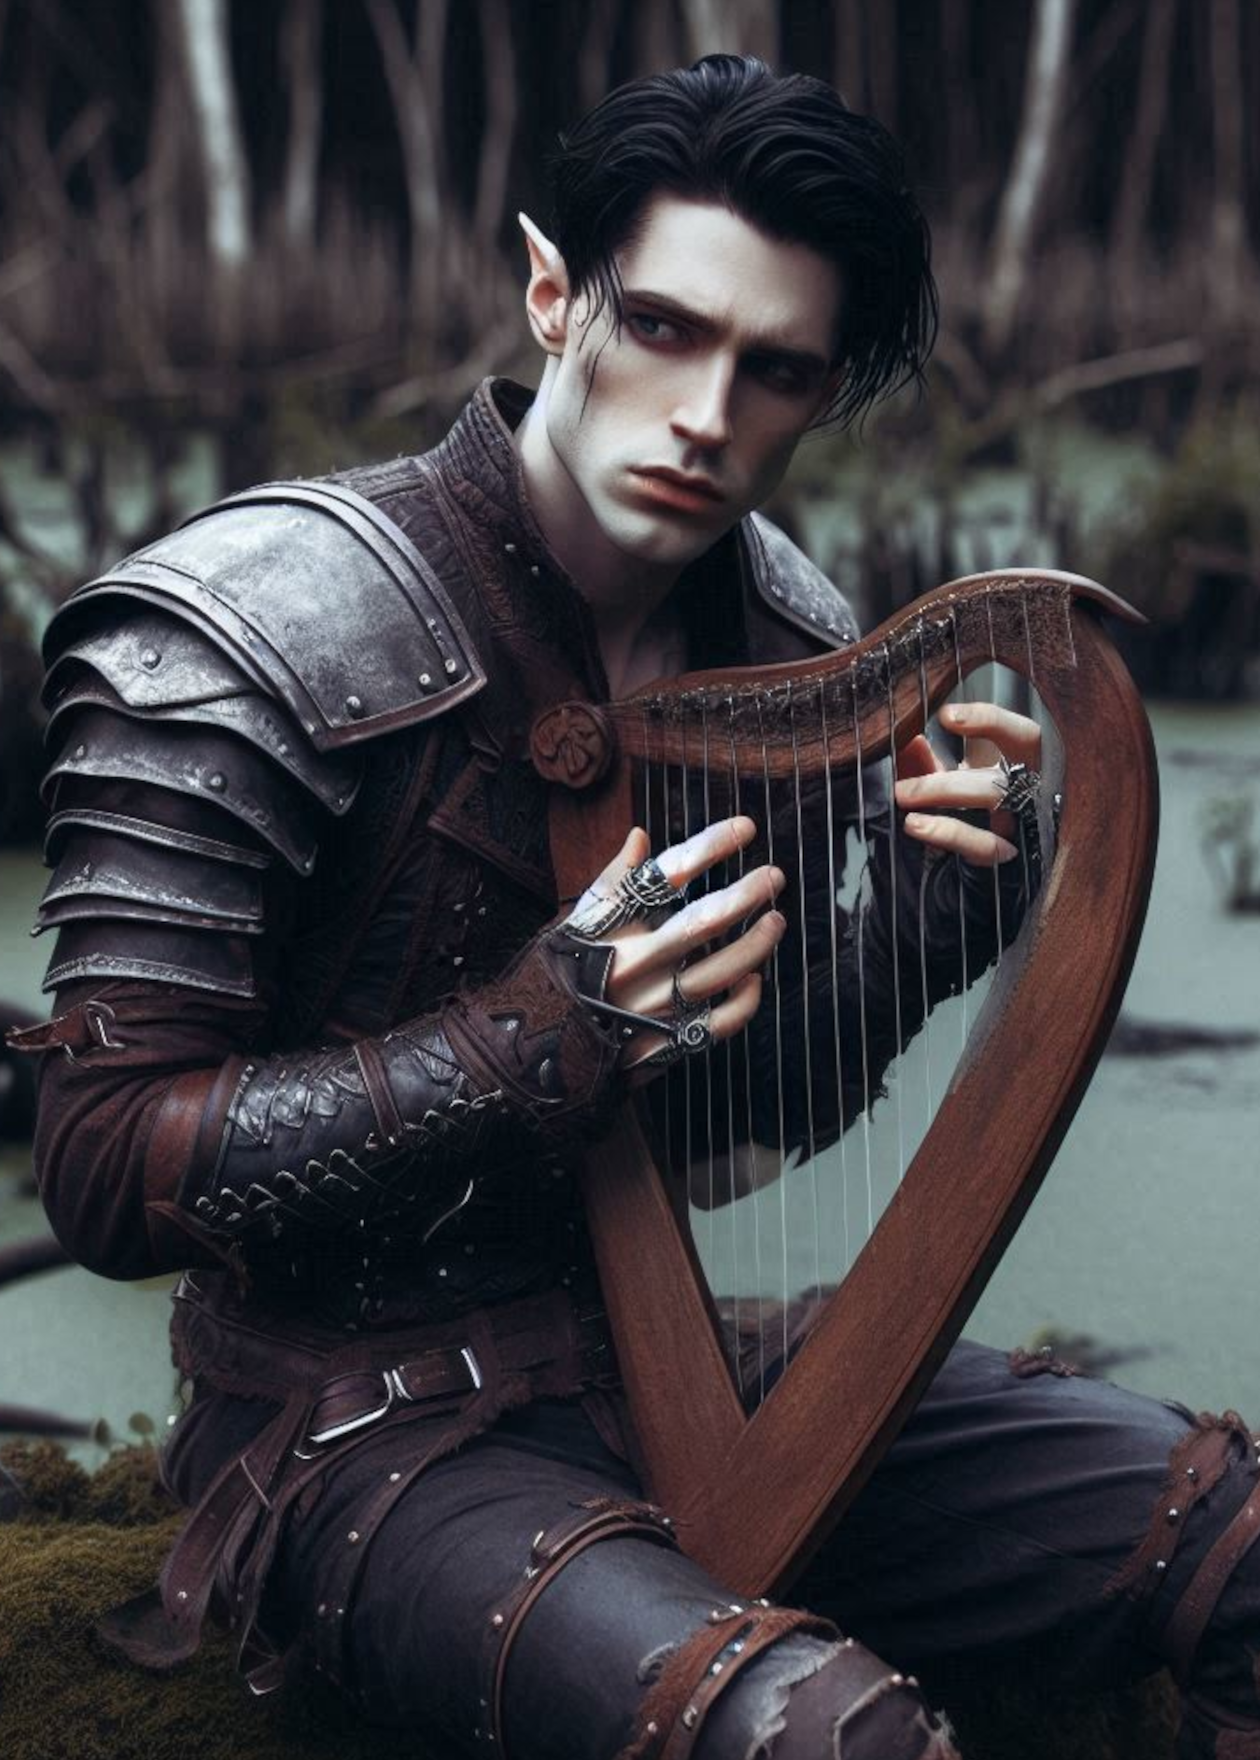
\includegraphics[width=63mm, height=88mm]{images/gon.png}};
    
    % Título
    \node[title, anchor=north west, minimum width=59mm](title) at (2,86) {Extra info of \textbf{Gon}};
    
    % PARTY
    \node[fill=parchment, opacity=0.7, text opacity=1, draw opacity=1, inner sep=0mm, anchor=north west, font=\sffamily\fontsize{8}{8.5}, draw=black, rounded corners=0.4mm, fit={(2,24) (30,2)}] (PARTY) {};
    \node[tag, anchor=east] at ([xshift=-0.5mm] PARTY.north east) {PARTY};
    \node[fit={(2,24) (12,2)}, fill=black, opacity=0.9, text opacity=1, draw opacity=1, inner sep=0mm, font=\sffamily\fontsize{4.5}{6}\selectfont, draw=black, rounded corners=0.4mm, align=left] (players) {};
    \node[anchor=west, align=right, text width=8mm, font=\color{white}\sffamily\fontsize{5}{7}\selectfont] (partyp) at (PARTY.west) {%
    Goodão\\[0.9em]
    Libaneiz\\[0.9em]
    Marcelo\\[0.9em]
    Nestor\\[0.9em]
    Pará\\[-0.4em]\phantom{.}
    };
    
    \node[anchor=west, align=left, text width=30mm,font=\sffamily\fontsize{5}{7}\selectfont] (partyc) at ([xshift=-1mm] partyp.east) {%
    \textbf{Arkvir}\\
    \vspace{-0.9mm}{\fontsize{4}{8}\selectfont Malkath, Tiefling Warlock}\\
    \textbf{Nora}\\
    \vspace{-0.9mm}{\fontsize{4}{8}\selectfont Tiefling Bard}\\
    \textbf{Griselda}\\
    \vspace{-0.9mm}{\fontsize{4}{8}\selectfont Kára, Aasimar Paladin}\\
    \textbf{Corvin}\\
    \vspace{-0.9mm}{\fontsize{4}{8}\selectfont Thorne, Human Bl Hunter}\\
    \textbf{Gartek}\\
    \vspace{-0.9mm}{\fontsize{4}{8}\selectfont Orc Barbarian}\\
    };
        
    % % PERS TRAITS
    % \node[fill=parchment, opacity=0.7, text opacity=1, draw opacity=1, inner sep=0mm, anchor=north west, font=\sffamily\fontsize{8}{8.5}, draw=black, rounded corners=0.4mm, fit={(29,24) (61,2)}] (PTRAITS) {};
    % \node[tag, anchor=east] at ([xshift=-0.5mm] PTRAITS.north east) {TEACHINGS};
    % \node[anchor=west, align=justify, text width=27mm, font=\sffamily\fontsize{4}{5}\selectfont] (traits) at (PTRAITS.west) {%
    % \faIcon[regular]{square}A disciplined mind brings happiness\\
    % \faIcon[regular]{square}If a man going down into a river is carried away by the current — how can he help others across?\\
    % \faIcon[regular]{square}You cannot travel the path until you have become the path itself.\\
    % \faIcon[regular]{square}There is no fear for one whose mind is not filled with desires\\
    % \faIcon[regular]{square}The root of suffering is attachment
    % };
    
    
    % DRUID
    \node[fill=parchment, opacity=0.7, text opacity=1, draw opacity=1, inner sep=0mm, anchor=north west, font=\sffamily\fontsize{8}{8.5}, draw=black, rounded corners=0.4mm, fit={(2,80) (61,52)}] (DRUID) {};
    \node[tag, anchor=west] at ([xshift=0.5mm] DRUID.north west) {DRUID};
    \node[anchor=north west, align=justify, yshift=-1mm, text width=27mm, font=\sffamily\fontsize{4.5}{5}\selectfont] (druid) at (DRUID.north west) {%
    \textbf{Druidic:} You know Druidic, the secret language of Druids. While learning this ancient tongue, you also unlocked the magic of communicating with animals;
    you always have the Speakwith Animals spell prepared. You can use Druidic to leave hidden messages. You and others who know Druidic automatically spot such a message.
    Others spot the message's presence with a successful DC 15 Intelligence (Investigation) check but can't decipher it without magic.\\[0.5em]
    % \textbf{Fey Ancestry:} You have advantage on saving throws you make to avoid or end the charmed condition on yourself.\\[0.5em]
    % \textbf{Long-limbed:} When you make a melee attack on your turn, your reach for it is 5 feet greater than normal.\\[0.5em]
    };
    
    \node[anchor=north west, align=justify, yshift=-1mm, text width=28mm, font=\sffamily\fontsize{4.5}{5}\selectfont] (druid) at ([xshift=28mm] DRUID.north west) {%
    \textbf{Wild Companion:} You can summon a nature spirit that assumes an animal form to aid you. As a Magic action, you can expend a spell slot or a use of Wild Shape to cast the Find Familiar spell without
    Material components. When you cast the spell in this way, the familiar is Fey and disappears when you finish a Long Rest.\\[0.5em]
    % \textbf{Wild Shape:} The power of nature allows you to assume the form of an animal. As a Bonus Action, you shape-shift into a Beast form that you have learned for this feature.
    % You stay in that form for a number of hours equal to half your Druid level or until you use Wild Shape again, have the Incapacitated condition, or die. You can also leave the form
    % early as a Bonus Action.\\[0.5em]
    % \textbf{Rules While Shape-Shifted:} While in a form, you retain your personality, memories, and ability to speak, and the following rules apply:\\
    % \textbf{Temporary Hit Points:} \sout{When you assume a Wild Shape form, you gain a number of Temporary Hit Points equal to your Druid level.}\\
    % \textbf{Game Statistics:} Your game statistics are replaced by the Beast's stat block, but you retain your creature type; Hit Points; Hit Point Dice; Intelligence, Wisdom,
    % and Charisma scores; class features; languages; and feats. You also retain your skill and saving throw proficiencies and use your Proficiency Bonus for them,
    % in addition to gaining the proficiencies ofthe creature. Ifa skill or saving throw modifier in the Beast's stat block is higher than yours, use the one in the stat block.\\
    % \textbf{No Spellcasting:} You can't cast spells, but shape- shifting doesn't break your Concentration or oth- erwise interfere with a spell you've already cast.\\
    % \textbf{Objects:} Your ability to handle objects is deter- mined by the form's limbs rather than your own. In addition, you choose whether your equipment falls in your space,
    % merges into your new form, or is worn by it. Worn equipment functions as normal, but the DM decides whether it's practical for the new form to wear a piece of equipment based
    % on the creature's size and shape. Your equipment doesn't change size or shape to match the new form, and any equipment that the new form can't wear must either fall to the ground
    % or merge with the form. Equipment that merges with the form has no effect while you're in that form.
    };
    
    % HUMAN
    \node[fill=parchment, opacity=0.7, text opacity=1, draw opacity=1, inner sep=0mm, anchor=north west, font=\sffamily\fontsize{8}{8.5}, draw=black, rounded corners=0.4mm, fit={(2,50) (30,40)}] (HUMAN) {};
    \node[tag, anchor=west] at ([xshift=0.5mm] HUMAN.north west) {HUMAN};
    \node[anchor=north west, align=justify, yshift=-1mm, text width=25mm, font=\sffamily\fontsize{4.5}{5}\selectfont] (human) at (HUMAN.north west) {%
    \textbf{Resourceful:} You gain Heroic Inspiration whenever you finish a Long Rest.\\[0.5em]
    };

    % % FIGHTER
    % \node[fill=parchment, opacity=0.7, text opacity=1, draw opacity=1, inner sep=0mm, anchor=north west, font=\sffamily\fontsize{8}{8.5}, draw=black, rounded corners=0.4mm, fit={(2,35) (61,9)}] (FIGHTER) {};
    % \node[tag, anchor=west] at ([xshift=0.5mm] FIGHTER.north west) {FIGHTER};
    % \node[anchor=north west, align=justify, yshift=-1mm, text width=27mm, font=\sffamily\fontsize{4.5}{5}\selectfont] (bugbear) at (FIGHTER.north west) {%
    % \textbf{Great weapon fighting (Fighting Style):} You have honed your martial prowess and gain a Fighting style feat of your choice.\\[0.5em]When you roll a 1 or 2 on damage die for an attack you make with a melee weapon that you arewielding with two hands, you can reroll the die, and you must use the new roll.\\[0.5em]The weapon must have the Two-Handed or versatile property to gain this benefit.\\[0.5em]
    % };
    
    % \node[anchor=north west, align=justify, yshift=-1mm, text width=28mm, font=\sffamily\fontsize{4.5}{5}\selectfont] (bugbear) at ([xshift=28mm] FIGHTER.north west) {%
    % \textbf{Weapon mastery:} Your training with weapons allows you to use the mastery property of three kinds of simple or martial weapons of your choice.\\[0.5em]Whenever you finish a long rest, you can practice weapon drills and change one of those weapon choices.\\[0.5em]Weapons: Halberd, pike and hand axe\\[0.5em]
    % };

    % FEATS
    \node[fill=parchment, opacity=0.7, text opacity=1, draw opacity=1, inner sep=0mm, anchor=north west, font=\sffamily\fontsize{8}{8.5}, draw=black, rounded corners=0.4mm, fit={(31,50) (61,2)}] (FEATS) {};
    \node[tag, anchor=west] at ([xshift=0.5mm] FEATS.north west) {FEATS};
    
    \node[anchor=north west, align=justify, yshift=-1mm, text width=27mm, font=\sffamily\fontsize{4.5}{5}\selectfont] (feats) at (FEATS.north west) {%
    \textbf{Magic Initiate (Druid):} Cantrips: Message, Poison Spray\\[0.5em]
    Level 1 Spell: Healing Word. You always have that spell prepared. You can cast it once without a spell slot, and you regain the ability to cast it in that way when you finish a Long Rest. You can also cast the spell using any spell slots you have.\\[0.5em]
    \textbf{Musician:} Instrument Training. You gain proficiency with three Musical Instruments of your choice: Lyre, Flute and Harp.\\[0.5em]
    Encouraging Song. As you finish a Short or Long Rest, you can play a song on a Musical Instrument with which you have proficiency and give Heroic Inspiration to allies who hear the song. The number of allies you can affect in this way equals your Proficiency Bonus.
\\[0.5em]
    };

    % EMPTY
    % \node[fill=parchment, opacity=0.7, text opacity=1, draw opacity=1, inner sep=0mm, anchor=north west, font=\sffamily\fontsize{8}{8.5}, draw=black, rounded corners=0.4mm, fit={(31,19) (61,2)}] (FIGHTER) {};
    % \node[tag, anchor=west] at ([xshift=0.5mm] FIGHTER.north west) {NOTES};

    % Borda
    \draw[line width = 0.5mm, black] (0,0) rectangle (63,88);
    
    \end{tikzpicture}%%
    